\documentclass[]{spie}  %>>> use for US letter paper
%\documentclass[a4paper]{spie}  %>>> use this instead for A4 paper
%\documentclass[nocompress]{spie}  %>>> to avoid compression of citations

\renewcommand{\baselinestretch}{1.0} % Change to 1.65 for double spacing
 
\usepackage{amsmath,amsfonts,amssymb}
\usepackage{graphicx,subcaption}
\usepackage[colorlinks=true, allcolors=blue]{hyperref}

%% For Theorems ...
\newtheorem{define}{Definition}[section]
% \newtheorem{theorem}{Theorem}[section]

\usepackage{graphicx,amsmath,amssymb,bbm,url}
\usepackage{algorithm}
\usepackage{algorithmic}
\usepackage{fullpage}

\newtheorem{lem}{Lemma}
\newtheorem{cor}{Corollary}
\newtheorem{thm}{Theorem}
\newtheorem{Def}{Definition}
\newtheorem{prop}{Proposition}

\def \vec{\overrightarrow}
\def \a {\mathbf a}
\def \b {\mathbf b}
\def \bar {\overline}
\def \ow {\text{otherwise}}
\def \x {\mathbf x}
\def \z {\mathbf z}
\def \y {\mathbf y}
\def \v {\mathbf v}
\def \C {\mathbbm{C}}
\def \Cd {\mathbbm{C}^d}
\def \R {\mathbbm{R}}
\def \Z {\mathbbm{Z}}
\def \N {\mathbbm{N}}
\def \M {\mathcal{M}}
\def \HS {\rm HS}
\def \X { X}
\def \Y { Y}
\def \m {\mathbf m}
\def \n {\mathbf n}
\def \P {\mathcal{P}}
\def \B {\mathcal{B}}
\def \one { \mathbbm{1}}
\def \e { \mathbbm{e}}
\def \i { \mathbbm{i}}
\def \jj {{j'}}
\def \elll {{\ell'}}
\def \sgn {{\rm sgn}}
\def \diag {{\rm diag}}
\def \supp {{\rm supp}}
\def \Span {{\rm span}}
\DeclareMathOperator{\Tr}{\rm Trace}
% Use more than 10 columns in bmatrix
\setcounter{MaxMatrixCols}{20}

% Reduce space between columns (for use with bmatrix and the 
% block circulant system matrix definition)
\def\SmallColSep{\setlength{\arraycolsep}{0.8\arraycolsep}}

\title{Phase Retrieval from Local Measurements in Two Dimensions}


\author[a]{Mark Iwen}
\author[b]{Brian Preskitt}
\author[b]{Rayan Saab}
\author[c]{Aditya Viswanathan}


\affil[a]{Department of Mathematics, and Department of Computational Mathematics, Science and Engineering (CMSE), Michigan State University, East Lansing, MI, 48824, USA}
\affil[b]{Department of Mathematics, University of California San Diego, La Jolla, 92093, USA}
\affil[c]{Department of Mathematics and Statistics, University of Michigan -- Dearborn, \newline 
  Dearborn, MI, 48128, USA}

\authorinfo{Further author information: (Send correspondence to Rayan Saab)\\Rayan Saab: E-mail:
rsaab@math.ucsd.edu}

% Option to view page numbers
\pagestyle{empty} % change to \pagestyle{plain} for page numbers
\setcounter{page}{301} % Set start page numbering at e.g. 301
 
\begin{document} 
\maketitle

\begin{abstract}
The phase retrieval problem has appeared in a multitude of applications for decades.  While ad hoc solutions have existed since the early 1970s, recent developments have provided algorithms that offer promising theoretical guarantees under increasingly realistic assumptions.  Motivated by ptychographic imaging, we generalize a recent result on phase retrieval of a one dimensional objective vector $\x \in \C^d$ to recover a two dimensional sample $Q \in \C^{d \times d}$ from phaseless measurements, using a tensor product formulation to extend the previous work.
\end{abstract}

% Include a list of keywords after the abstract 
\keywords{Phase Retrieval, Local Measurements, Two Dimensional Imaging, Ptychography, Fast Algorithms}

\section{Introduction}

Consider the problem of recovering a 2-dimensional image $Q \in \C^{d \times d}$ from measurements of the form \begin{equation} y_k = \left| \sum_{i,j = 1}^d Q_{ij} A^{(k)}_{ij} \right|^2, \label{eq:phaseRetrieval}\end{equation} where $A^{(k)}$ is a collection of known measurement vectors.  This is known as the \emph{phase retrieval problem}\cite{gerchberg1972practical,walther1963question}, as the system \eqref{eq:phaseRetrieval} may be seen as a system of linear equations in the variables $Q_{ij}$ wherein the phases of the measurements $y_k$ have been discarded by the componentwise $|\cdot|^2$ operation.   This problem appears in a number of imaging scenarios, for example X-ray crystallography\cite{millane1990phase}, electron microscopy\cite{ferwerda1975electron}, and ptychography\cite{rodenburg2008ptychography}, which shall be the primary motivation for the technique presented here.

In ptychography, a light source applies a sharply focused beam onto a sample, which scatters the incoming ray onto an array of intensity sensors behind.  The light source is then shifted and applied to different parts of the sample to obtain the measurement redundancy necessary to resolve an accurate image from this data.  We model this as
\begin{equation}
\left| \left(\mathcal{F}\left[S_{x_0, y_0}a \cdot q\right] \right)(u,v) \right|^2, ~~(u,v) \in \Omega \subset \mathbbm{R}^2,~~(x_0, y_0) \in \mathcal{L} \subset [0,1]^2,
\label{def:Prob_Continuous}
\end{equation}
where $\mathcal{F}$ denotes the 2 dimensional Fourier transform (arising from the optical diffraction), $a:\mathbbm{R}^2 \rightarrow \mathbbm{C}$ is a known function representing the intensity of the illumination, $S_{x_0, y_0}$ is a shift operator defined by $\left(S_{x_0, y_0}a\right)(x,y) := a(x-x_0, y-y_0)$, $\Omega$ is a finite set of sampled frequencies, and $\mathcal{L}$ is a finite set of shifts.  %% Therefore, \eqref{def:Prob_Continuous} describes a collection of measurements obtained by applying a single illumination pattern $a$ to the sample $q$ from various positions; the Fourier transform appears due to the diffractive scattering of the light through the sample\cite{rodenburg2008ptychography}.
As a typical characteristic of ptychography is that the beam is sharply focused, we assume that $a$ is compactly supported within a smaller region $[0, \delta']^2$ for $\delta' \ll 1$.  %% Herein we will make the further assumption that all the utilized shifts of $q$ also have their supports contained in $[0,1]^2$.  That is, that
%% $$\bigcup_{(x_0, y_0) \in \mathcal{L}} \supp\left( S_{x_0, y_0}q \right) \subseteq [0,1]^2$$
%% holds.  Note that an analogous assumption can always be achieved by dilating $[0,1]^2$.

Discretizing \eqref{def:Prob_Continuous} using periodic boundary conditions yields a finite dimensional problem aimed at recovering an unknown matrix $Q \in \mathbbm{C}^{d \times d}$ from phaseless measurements of the form
\begin{equation}
y_{(\ell, \ell', u, v)} = \left| \frac{1}{d^2} \sum^d_{j=1} \sum^d_{k=1} Q_{j,k} \left(S_{\ell}AS^*_{\ell'}\right)_{j,k} \e^{\frac{-2\pi \i}{d}(ju + kv)} \right|^2 = \left| \frac{1}{d^2} \sum_{j=1}^d \sum_{k=1}^d Q_{j,k}\left(W^{-u} S_{\ell}AS^*_{\ell'}W^{-v}\right)_{j,k} \right|^2.
\label{def:Prob_Disc_Gen}
\end{equation}
Here $A \in \mathbbm{C}^{d \times d}$ is the discretization of our illuminating beam, $S_\ell \in \mathbbm{R}^{d \times d}$ is the discrete circular shift operator defined by $(S_\ell \x)_j := x_{j-\ell ~{\rm mod}~ d}$ for all $\x \in \mathbbm{C}^d$ and $j,\ell \in [d] := \{ 1, \dots, d\}$, and $W = \diag(\e^{\frac{2 \pi \i k}{d}})$ is the modulation operator.  Also, $(\ell, \ell', u, v) \in \mathcal{L}^2 \times \Omega^2$ where $\mathcal{L}, \Omega \subset [d]$ are the index sets for the shifts and frequencies, respectively.  Herein we will make the simplifying assumption that our original illuminating beam function $a$ is not only sharply focused, but also separable.  Specifically, we assume that the discretized measurement matrix takes the form $$\frac{1}{d^2} A := \a \b^*$$ where $\a,\b \in \mathbbm{C}^d$ both have $\supp(\a), \supp(\b) \subset [\delta]$ for some $\delta \in \mathbbm{Z}^+$ with $\delta \ll d$. We leave the generalization to "non-separable" matrices $A$ to future work. 

%% Using the small support and separability of $\frac{1}{d^2} A := \a \b^*$ we can now rewrite the measurements \eqref{def:Prob_Disc_Gen} as
%% \begin{align}
%% \left| \sum^\delta_{j=1} \sum^\delta_{k=1} a_j \overline{b_k} \left(S_{\ell}QS^*_{\ell'}\right)_{j,k} \e^{\frac{-2\pi \i}{d}(ju + kv)} \right|^2 &= \left| \sum^\delta_{j=1} \sum^\delta_{k=1} \overline{\overline{a_j}\e^{\frac{2 \pi \i j u}{d}}  b_k \e^{\frac{2 \pi \i k v}{d}}} \left(S_{\ell}QS^*_{\ell'}\right)_{j,k} \right|^2 \nonumber \\
%% &= \left| \left\langle S_{\ell}QS^*_{\ell'}, \a_u \b^*_v \right\rangle_{\HS} \right|^2
%% \label{Prob_Disc_Sep1}
%% \end{align}
We can now rewrite the measurements \eqref{def:Prob_Disc_Gen} as%
\begin{align}
y_{(\ell, \ell', u, v)} &=  \left| \frac{1}{d^2} \langle Q, W^{-u} S_\ell A S_{\ell'}^* W^{-v} \rangle_{\HS}\right|^2 \\ &= \left| \frac{1}{d^2} \e^{\frac{2 \pi \i( \ell u + \ell' v)}{d}} \langle Q, S_\ell W^{-u} A W^{-v} S_{\ell'}^* \rangle_{\HS}\right|^2 \nonumber \\
  &= \left|\langle Q, S_\ell W^{-u} \a \b^* W^{-v} S_{\ell'}^* \rangle_{\HS}\right|^2 \nonumber \\
  &= \left|\langle Q, S_\ell \a_u (S_{\ell'} \b_v)^* \rangle_{\HS}\right|^2
  \label{eq:HS_meas}
\end{align}%
where $\a_u, \b_v \in \mathbbm{C}^d$ are defined by $\left( a_u \right)_j := \e^{\frac{-2 \pi \i j u}{d}} a_j$ and $\left( b_v \right)_k := \e^{\frac{2 \pi \i k v}{d}} b_k$ for all $j,k \in [d]$.%%   Continuing to rewrite \eqref{Prob_Disc_Sep1} we can now see that our discretized measurements will all take the form of 
%% \begin{equation}
%% \left| \left\langle S_{\ell}QS^*_{\ell'}, \a_u \b^*_v \right\rangle_{\HS} \right|^2 = \left| \left\langle Q, S_\ell^* \a_u \b^*_v S_{\ell'} \right\rangle_{\HS} \right|^2 = \left| \left\langle Q, S^*_{\ell} \a_u \left(S^*_{\ell'} \b_v \right)^* \right\rangle_{\HS} \right|^2
%% \label{Prob_Disc}
%% \end{equation}
%% for a finite set of frequencies $(u,v) \in \Omega \subset [d]^2$ and shifts $(\ell,\ell') \in \mathcal{L} \subseteq [d] \times [d]$.

Motivated by the above model of ptychographic imaging, we propose a new efficient numerical scheme for solving general discrete phase retrieval problems using measurements of type \eqref{eq:HS_meas} herein.  After a brief discussion of notation, we will outline our proposed method in \S\ref{sec:TheMethod} below, along with a basic analysis guaranteeing the success of the method under appropriate assumptions.  A preliminary numerical evaluation of the method is then presented in \S\ref{sec:Numerics}.

\subsection*{Notation and Preliminaries}

 For any $k \in \N,$ we define $[k] := \{1, 2, \ldots, k\}$.  For $i, j \in \N, e_i$ represents the standard basis vector and $E_{ij} = e_i e_j^*$; the dimensions of such an $E_{ij}$ will always be clear from context.  For a matrix $A \in \C^{m \times n},$ $$\vec{A} := (a_{11}, a_{21}, \ldots, a_{m1}, \ldots, a_{mn})^T \in \C^{mn}$$ denotes the column-major vectorization of $A$.  $A \otimes B$ for arbitrary matrices denotes the standard Kronecker product.  We remark that $\vec{\a\b^*} = \bar{\b} \otimes \a$, and in particular%
\begin{equation}
  \vec{E_{jk}} \vec{E_{j'k'}}^* = \vec{e_j e_k^*} \vec{e_{j'} e_{k'}^*} = (e_k \otimes e_j) (e_{k'} \otimes e_{j'})^* = (e_k e_{k'}^*) \otimes (e_j e_{j'}^*) = E_{kk'} \otimes E_{jj'}.
  \label{id:kronsimp}
\end{equation} We let $\langle A, B \rangle_{\HS} := \Tr(A^* B) = \langle \vec{A}, \vec{B} \rangle$ denote the Hilbert-Schmidt inner product on $\C^{n \times n}$ and remark that, for $\x, \y \in \C^n,$ %
  \begin{equation}%
    |\langle \x, \y \rangle |^2 = \langle \x \x^*, \y \y^* \rangle_{\HS}.%
    \label{id:quadprod}%
  \end{equation}%
%
  In addition, indices are always taken modulo $d$, and for indices we define \begin{equation} |i - j| := \min \{k : k \equiv i - j \mod d \ \text{or} \ k \equiv j - i \mod d, k \ge 0\} \label{eq:modabs} \end{equation} so that $|i - j| < \ell$ implies that there is some $k, |k| < \ell$ such that $j + k \equiv i \mod d$.

\section{An Efficient Method for Solving the Discrete 2D Phase Retrieval Problem}
\label{sec:TheMethod}
Our recovery method, outlined in Algorithm \ref{Alg1}, aims to approximate an image $Q\in \C^{d\times d}$ from phaseless measurements of the form \eqref{eq:HS_meas}.    
%
%
\begin{algorithm}[b!]
\renewcommand{\algorithmicrequire}{\textbf{Input:}}
\renewcommand{\algorithmicensure}{\textbf{Output:}}
\caption{Two Dimensional Phase Retrieval from Local Measurements}
\label{Alg1}
\begin{algorithmic}[1]
    \REQUIRE Measurements $\y\in \mathbbm{R}^D$ as per \eqref{def:Measurements}
    \ENSURE $X \in \mathbbm{C}^{d \times d}$ with $X \approx \mathbbm{e}^{-\mathbbm{i} \theta} Q$ for some $\theta \in [0, 2 \pi]$ 
    \STATE Compute the Hermitian matrix $P = \Big( \left(\mathcal{M} \big|_{\mathcal{P}}\right)^{-1} {\bf y}\Big)/2 + \Big( \left(\mathcal{M} \big|_{\mathcal{P}}\right)^{-1} {\bf y}\Big)^*/2  \in \mathcal{P}\left(\mathbbm{C}^{d^2\times d^2}\right)$ as an estimate of $\mathcal{P} \left( \vec{Q} \vec{Q}^* \right)$.  $\mathcal{M}$ and $\mathcal{P}$ are as defined in \eqref{Def:Measure_Operator} and \S\ref{sec:linear}.
    \STATE Form the matrix of phases, $\widetilde{P} \in \mathcal{P}\left(\mathbbm{C}^{d^2\times d^2}\right)$, by normalizing the non-zero entries of $P$.
    \STATE Compute the principal eigenvector of $\widetilde{P}$ and use it to compute $U_{j,k} \approx \sgn\left( Q_{j,k}\right) ~\forall j,k \in [d]$ as per \S\ref{sec:Getphases}.
    \STATE Use the diagonal entries of $P$ to compute $M_{j,k} \approx \left| Q_{j,k} \right|^2$ for all $j,k \in [d]$ as per \S\ref{sec:Getmags}.
    \STATE Set $X_{j,k} = \sqrt{M_{j,k}} \cdot U_{j,k}$ for all $j,k \in [d]$ to form $X$
    %\STATE Set $\x = W^* \widetilde{\x}$ 
    \end{algorithmic}
\end{algorithm}
%
%
%
In this analysis, we generalize by considering a collection of measurements given by 
\begin{equation}
y_{(\ell,\ell',u,v)} := \left| \left\langle Q, S^*_{\ell} \a_u \left(S^*_{\ell'} \b_v \right)^* \right\rangle_{\HS} \right|^2
\label{def:Measurements}
\end{equation}
for all $(\ell,\ell',u,v) \in [d]^2 \times\Omega^2$ where $\Omega \subset [d]$ has $|\Omega| = 2\delta-1$.  Thus, we collect a total of $D := (2\delta-1)^2 \cdot d^2 $ measurements where each measurement is due to a vertical and horizontal shift of a rank one illumination pattern $\a_u \b_v^* \in \mathbbm{C}^{d \times d}$.  Unlike the example of ptychography, in this analysis we do not require that $\a_u$ and $\b_v$ are modulations of fixed vectors $\a$ and $\b$; rather $\a_u$ and $\b_v$ may be chosen arbitrarily (to allow more general setups).  However, we do assume that our measurements are \emph{local} in the sense that $\supp(\a), \supp(\b) \subset [\delta].$ %$\left(a_u\right)_j = \left(b_v \right)_j = 0$ for all $j \in [d] \setminus [\delta]$ and all $(u,v) \in \Omega^2$. %% \footnote{For any $n \in \mathbbm{Z}^+$ we will define $[n] := \{ 1, 2, 3, \dots, n \} \subset \mathbbm{Z}^+$.}  
 Recall that $\delta \ll d$, so the total number of measurements $D$ is essentially linear in the problem size.
 % Our recovery algorithm is a variant of  the BlockPR agorithm\cite{iwen2016fast,iwen2016phase}.

Algorithm \ref{Alg1} consists of first rephrasing the system \eqref{def:Measurements} as a linear system on the space of $d^2 \times d^2$ matrices (following Candes, et al. \cite{candes2013phaselift}), and then estimating a projection $\mathcal{P}( \vec{Q}\vec{Q}^*)$ of the rank one matrix $\vec{Q}\vec{Q}^*$ from this system.  This process is described in \S\ref{sec:linear}.  In \S\S\ref{sec:Getphases}-\ref{sec:Getmags} we show how the magnitudes of the entries of $Q$ are estimated directly from $\mathcal{P}(\vec{Q}\vec{Q}^*)$ and their phases are found from solving an eigenvector problem.  Together, the magnitude and phase estimates provide an approximation of $Q$.

%  \cite{candes2013phaselift} of the discrete 2D phase retrieval problem from local measurements of type \eqref{Prob_Disc}.

\subsection{The Linear Measurement Operator $\mathcal{M}$ and Its Inverse}
\label{sec:linear}
To produce the linear system of step 1, we observe that
\begin{align*}%
y_{(\ell,\ell',u,v)} &= \left| \left\langle Q, S^*_{\ell} \a_u \left(S^*_{\ell'} \b_v \right)^* \right\rangle_{\HS} \right|^2 = |\langle \vec{Q}, S_{\ell'}^* \bar{\b_u} \otimes S_{\ell}^* \a_v \rangle_{\HS} |^2 \\%
&= \left\langle  \vec{Q} \vec{Q}^*, ~\left(S_{\ell'}^* \bar{\b_u} \otimes S_{\ell}^* \a_v\right) \left(S_{\ell'}^* \bar{\b_u} \otimes S_{\ell}^* \a_v\right)^* \right\rangle_{\HS},
\end{align*} %With identity \eqref{id:quadprod} %$|\langle \x, \y \rangle|^2 = (x^*y) (y^* x) = \Tr\left(x^* y y^* x \right) = \Tr(x x^* y y^*) = \langle x x^*, y y^* \rangle,$
%$|\langle \x, \y \rangle |^2 = \langle \x \x^*, \y \y^* \rangle_{\HS}$ for arbitrary $\x, \y \in \C^n$,
%we can further see that $$y_{(\ell,\ell',u,v)} = \left\langle  \vec{Q} \left( \vec{Q} \right)^*, ~S_{\ell'}^* \bar{\b_u} \otimes S_{\ell}^* \a_v \left(S_{\ell'}^* \bar{\b_u} \otimes S_{\ell}^* \a_v\right)^* \right\rangle$$
%% \begin{align*}
%% y_{(\ell,\ell',u,v)} &=\left\langle S^*_{\ell} \overline{\a_u} \otimes S^*_{\ell'} \b_v, \vec{Q^*} \right\rangle \overline{\left\langle S^*_{\ell} \overline{\a_u} \otimes S^*_{\ell'} \b_v, \vec{Q^*} \right\rangle } \\
%% &= \left( \vec{Q^*} \right)^* S^*_{\ell} \overline{\a_u} \otimes S^*_{\ell'} \b_v \left( S^*_{\ell} \overline{\a_u} \otimes S^*_{\ell'} \b_v \right)^* \vec{Q^*} \\
%% &= {\rm Trace}\left( \vec{Q^*} \left( \vec{Q^*} \right)^* S^*_{\ell} \overline{\a_u} \otimes S^*_{\ell'} \b_v \left( S^*_{\ell} \overline{\a_u} \otimes S^*_{\ell'} \b_v \right)^* \right)\\
%% &=\left\langle  \vec{Q^*} \left( \vec{Q^*} \right)^*, ~S^*_{\ell} \overline{\a_u} \otimes S^*_{\ell'} \b_v \left( S^*_{\ell} \overline{\a_u} \otimes S^*_{\ell'} \b_v \right)^*\right\rangle_{\HS}.
%% \end{align*}
which allows us to naturally define $\mathcal{M}: \mathbbm{C}^{d^2 \times d^2} \mapsto \mathbbm{R}^D$ as the linear measurement operator given by 
\begin{equation}
\left(\mathcal{M}(Z) \right)_{(\ell,\ell',u,v)} := \left\langle  Z, ~\left(S_{\ell'}^* \bar{\b_u} \otimes S_{\ell}^* \a_v\right) \left(S_{\ell'}^* \bar{\b_u} \otimes S_{\ell}^* \a_v\right)^*\right\rangle_{\HS} = \left\langle Z, ~\left(S_{\ell'}^* \bar{\b_u}\bar{\b_u}^* S_{\ell'}\right) \otimes \left(S_\ell^* \a_v \a_v^* S_\ell \right) \right\rangle_{\HS},
\label{Def:Measure_Operator}
\end{equation}
so that $\y = \mathcal{M}(\vec{Q} \vec{Q}^*)$.  This allows us to solve for $\P(\vec{Q} \vec{Q}^*)$, the projection of $\vec{Q} \vec{Q}^*$ onto the rowspace $\P(\C^{d^2 \times d^2})$ of $\M$.  For clarity, we will abbreviate $\P(\C^{d^2 \times d^2})$ as $\P$, identifying this subspace with its orthogonal projection operator.

We observe that the local supports of $\a_u$ and $\b_v$ ensure that $\mathcal{M}( \vec{E_{j,k}} \vec{E_{j',k'}}^*) = {\bf 0}$ whenever either $|j - j'| \geq \delta$ or $|k - k'| \geq \delta$ holds (this is clear from \eqref{Def:Measure_Operator} and \eqref{id:kronsimp}).  As a result we can see that $\P \subset \B$ where \begin{equation} \B := \Span\{ \vec{E_{j,k}} \vec{E_{j',k'}}^* ~{\bf \big |}~  |j - j'| < \delta, |k - k'| < \delta \}. \label{eq:B}\end{equation}  %% \footnote{Note that projection onto $\Span(\B)$ can also be described as a restriction operator onto the indices associated with the elements of $\B$.  Our periodic boundary conditions also imply that, e.g., $|j - j'| < \delta \Leftrightarrow \exists h \in \mathbbm{Z}~{\rm with}~ |h| < \delta~{\rm s.t.}~j' + h \equiv j ~{\rm mod}~d$.}
In steps 2-4 of Algorithm \ref{Alg1}, recovery of $Q$ from $\P(\vec{Q} \vec{Q}^*)$ relies on having $\P = \B$ exactly; we say in such a case that $\M|_\B$ is invertible.  Clearly, the invertibility of $\M$ over $\B$ will depend on our choice of $\a$ and $\b$.  We prove the following proposition, a corollary of which identifies pairs $\a, \b$ which produce an invertible linear system:
\begin{prop}
  Let $T_\delta : \C^{d \times d} \to \C^{d \times d}$ be the operator given by $$T_\delta(X)_{ij} = \left\{\begin{array}{r@{,\quad}l}
  X_{ij} & |i - j| < \delta \mod d \\
  0 & \text{otherwise}\end{array}\right..$$
  If the space $T_{\delta}(\C^{d \times d})$ is spanned by the collection $\{\a_j \a_j^*\}_{j=1}^K$, then $\B$ is spanned by $$\{(\a_j \otimes \a_{j'}) (\a_j \otimes \a_{j'})^*\}_{(j, j') \in [K]^2} = \{(\a_j \a_j^*) \otimes (\a_{j'} \a_{j'}^*)\}_{(j, j') \in [K]^2}.$$
  \label{prop:kronspan}
\end{prop}
%
\begin{proof}
  By \eqref{id:kronsimp}, it suffices to show that $$(e_k e_{k'}^*) \otimes (e_j e_{j'}^*) \in \Span\{(\a_n \a_n^*) \otimes (\a_{n'} \a_{n'}^*)\}_{(n, n') \in [K]^2}$$ for any $|j - j'|, |k - k'| < \delta$.  Indeed, we have that $\{E_{jj'} : |j - j'| < \delta \mod d\}$ forms a basis for $T_\delta(\C^{d \times d})$, so $E_{j j'}, E_{k k'} \in \Span\{\a_n \a_n^*\}_{n \in [K]}$ and $$(e_k e_{k'}^*) \otimes (e_j e_{j'}^*) \in \Span\{(\a_n \a_n^*) \otimes (\a_{n'} \a_{n'}^*)\}_{(n, n') \in [K]^2}.$$
\end{proof}

In Theorem 4 of Iwen et al.\cite{iwen2016fast}, an illumination function $\a \in \C^d$ with $\supp(\a) \subset [\delta]$ is offered such that $\{S_\ell \a_u \a_u^* S_\ell^*\}_{(\ell, u) \in [d]^2}$ spans $T_\delta(\C^{d \times d})$.  By proposition \ref{prop:kronspan}, this gives the following corollary.

\begin{cor}
  Choose a constant $a \in [4, \infty)$ and let the vectors $\a_\ell$ be defined by $(\a_\ell)_k = \dfrac{\e^{-k / a} \cdot \e^{\frac{2 \pi \i k}{2\delta - 1}}}{\sqrt[4]{2 \delta - 1}} \cdot \mathbbm{1}_{k \le \delta}$.  Then $$\{S_\ell^* \bar{\a_u} \bar{\a_u}^* S_\ell \otimes S_{\ell'}^* \a_v \a_v^* S_{\ell'}\}_{(u, v, \ell, \ell') \in [d]^2 \times p[2 \delta - 1]^2}$$ spans $\B$.
    %% $$(\a_\ell)_k = \left\{\begin{array}{c@{\ }l}
    %% \dfrac{e^{-k / a}}{\sqrt[4]{2 \delta - 1} \cdot e^{\frac{2 \pi i (k - 1)(\ell - 1)}{2 \delta - 1}} & \text{if} \ k \le \delta \\
      %%   0 & \text{otherwise}\end{array}\right.$$
      \label{cor:fourier_masks}
\end{cor}

Towards application in ptychography, we remark that the vectors listed in \ref{cor:fourier_masks} may be achieved as modulations of $\a$ with $\a_k = \e^{-k/a} / \sqrt[4]{2 \delta - 1}$ if $2 \delta - 1$ divides $d$.  This condition may be met by zero padding $Q$ as needed.  The next corollary provides an example of measurement vectors that span $\B$, but are not produced by modulations.
The authors of this work  also constructed another collection of vectors (Example 2 of the previous work \cite{iwen2016phase}), yielding another spanning set for $T_\delta$. By the same reasoning as above, we have the following corollary. 
\begin{cor}
  Let $\a_1 = e_1$ and for $k \in [\delta], \a_{2k} = e_1 + e_k, \a_{2k + 1} = e_1 + \i e_k.$  Then $$\Span\left(S_\ell \overline{\a_u \a_{u}^*} S_{\ell} \otimes S_{\ell'} \a_v \a_v^* S_{\ell'}^* \right) = \B.$$ \label{cor:sparse_masks}
\end{cor}

\

\subsection{Computing the Phases of the Entries of $Q$ after Inverting $\mathcal{M} \big|_{\B}$}
\label{sec:Getphases}

Assuming that $\P = \B$ (as defined in \eqref{eq:B}; this condition may be satisfied according to Corollaries \ref{cor:fourier_masks} and \ref{cor:sparse_masks}) so that we can recover $\P ( \vec{Q} \vec{Q}^* ) = \B ( \vec{Q} \vec{Q}^* )$ from our measurements $\y$, we are still left with the problem of how to recover $\vec{Q}$ from $\B ( \vec{Q} \vec{Q}^* )$.  Our first step in solving for $\vec{Q}$ will be to compute all the phases of the entries of $\vec{Q}$ from $\B(\vec{Q} \vec{Q}^*)$.  Thankfully, this can be solved as an angular synchronization problem\cite{singer2011angular} as in BlockPR.\cite{viswanathana2015fast,iwen2016phase}  Let $\one \in \mathbbm{C}^{d^2 \times d^2}$ be the matrix of all ones, and $\sgn: \mathbbm{C} \mapsto  \mathbbm{C}$ be 
$$\sgn(z) = \left\{\begin{array}{r@{,\qquad}l} \dfrac{z}{|z|} & z \neq 0 \\ 1 & \text{otherwise} \end{array}\right..$$
We now define $\widetilde{Q} \in \mathbbm{C}^{d^2 \times d^2}$ by $\widetilde{Q} = \B(\sgn(\vec{Q} \vec{Q}^*))$ (i.e. $\widetilde{Q}$ is $\B(\vec{Q}\vec{Q}^*)$ with its non-zero entries normalized). %
%% \begin{equation}
%% \widetilde{Q}_{j,k} := \left\{\begin{array}{r@{,\qquad}l} \sgn \left( \left[ \B \left( \vec{Q} \left( \vec{Q} \right)^* \right) \right]_{j,k} \right) & \left[ \B \left( \one \one^* \right) \right]_{j,k} \neq 0 \\ 0~~~~~~~~~~~~~~~~~~~~~~~~ & \text{otherwise} \end{array}\right..
%% \label{def:Qtilde}
%% \end{equation}
As we shall see, the principal eigenvector of $\widetilde{Q}$ will provide us with all of the phases of the entries of $\vec{Q}$.

Indeed, we may note that
\begin{equation}
\widetilde{Q} = \diag \left( \sgn \left( \vec{Q} \right) \right) \B \left( \one \one^* \right) \diag \left( \overline{\sgn \left( \vec{Q} \right)} \right)
\label{equ:Qtilde_partial_factor}
\end{equation}
where $\sgn$ is applied component-wise to vectors, and where $\diag(\x)  \in \mathbbm{C}^{d^2 \times d^2}$ is diagonal with $\left(\diag(\x)\right)_{j,j} := x_j$ for all $\x \in \mathbbm{C}^{d^2}$ and $j \in [d^2]$.  As $\diag(\sgn(\cdot))$ always produces a unitary diagonal matrix, we can further see that the spectral structure of $\widetilde{Q}$ is determined by $\B \left( \one \one^* \right)$.  The following theorem completely characterizes the eigenvalues and eigenvectors of $\B \left( \one \one^* \right)$.

\begin{thm} 
Let $F \in \mathbbm{C}^{d \times d}$ be the unitary discrete Fourier transform matrix with $F_{j,k} := \frac{1}{\sqrt{d}} \e^{2 \pi \i \frac{(j-1)(k-1)}{d}} ~\forall j,k \in [d]$, and let $D \in \mathbbm{C}^{d \times d}$ be the diagonal matrix with $D_{j,j} = 1 + 2 \sum^{\delta-1}_{k=1} \cos \left( \frac{2 \pi (j-1)k}{d} \right)~\forall j \in [d]$.  Then,
$$\B \left( \one \one^* \right) = \left( F \otimes F \right) \left( D \otimes D \right) \left( F \otimes F \right)^*.$$
In particular, the principal eigenvector of $\B \left( \one \one^* \right)$ is $\one$ and its associated eigenvector is $(2 \delta - 1)^2$. 
\label{thm:Factorized_P11}
\end{thm}

\begin{proof}
From the definition of $\B$ we have that 
\begin{align*}
  \B \left( \one \one^* \right) &= \sum^d_{j=1} ~\sum_{|j - j'| < \delta} ~\sum^d_{k=1} ~\sum_{|k - k'| < \delta}\vec{E_{j,k}} \left(\vec{E_{j',k'}} \right)^* \\
  &= \sum^d_{j=1} ~\sum_{|j - j'| < \delta} ~\sum^d_{k=1} ~\sum_{|k - k'| < \delta} E_{kk'} \otimes E_{jj'} \\
  &= \left(\sum^d_{k=1} ~\sum_{|k - k'| < \delta} E_{kk'}\right) \otimes \left( \sum^d_{j=1} ~\sum_{|j - j'| < \delta} E_{jj'} \right) \\
  &= T_\delta\left(\one \one^*\right) \otimes T_\delta \left(\one \one^*\right).
\end{align*}
Thankfully the eigenvectors and eigenvalues of $T_\delta(\one \one^*)$ are known (see Lemma 1 of our previous work\cite{iwen2016phase}).  Specifically, $T_\delta(\one \one^*) = F D F^*$ which then yields the desired result by Theorem 4.2.12 of Horn and Johnson\cite{horn1991topics}.
\end{proof}

Theorem~\ref{thm:Factorized_P11} in combination with \eqref{equ:Qtilde_partial_factor} makes it clear that $\sgn (\vec{Q})$ will be the principal eigenvector of $\widetilde{Q}$.  As a result, we can rapidly compute the phases of all the entries of $\vec{Q}$ by using, e.g., a shifted inverse power method\cite{trefethen1997numerical} in order to compute the eigenvector of $\widetilde{Q}$ corresponding to the leading eigenvalue $(2 \delta - 1)^2$. 

\subsection{Computing the Magnitudes of the Entries of $Q$ after Inverting $\mathcal{M} \big|_{\B}$}
\label{sec:Getmags}

Having found the phases of each entry of $\vec{Q}$ using $\B ( \vec{Q} \vec{Q}^* )$, it only remains to find each entry's magnitude as well.  This is comparably easy to achieve.  Note that $\B$ trivially contains $\vec{E_{j,k}}\vec{E_{j,k}}^* = e_ke_k^* \otimes e_je_j^*$ for all $j, k \in [d]$, so $\B ( \vec{Q} \vec{Q}^* )$ is guaranteed to always provide the diagonal entries of $\vec{Q} \vec{Q}^*$, which are exactly the squared magnitudes of the entries of $\vec{Q}$.  Combined with the phase information recovered in step 2 of Algorithm \ref{Alg1}, we are finally able to reconstruct every entry of $\vec{Q}$ up to a global phase as in step 5.


\section{Numerical Evaluation}
\label{sec:Numerics}
We will now demonstrate the efficiency and robustness of Algorithm~\ref{Alg1}. Figures
\ref{fig:recon} and \ref{fig:recon_msu} plot the reconstruction of two $256\times 256$ test 
images (shown in Figures \ref{fig:true} and \ref{fig:true_msu} respectively) from squared
magnitude local measurements of the type described in (\ref{def:Prob_Disc_Gen}). Here both $\a$ and $\b$ are
chosen to be the {\em deterministic} measurement vectors of Corollary 2, detailed in Example 2 of \cite[Section
2]{iwen2016phase}, with $\delta$ chosen to be $2$. The reconstructions were computed using an
implementation of Algorithm~\ref{Alg1} in Matlab$^\circledR$ running on a Laptop computer (Ubuntu
Linux 16.04 {\tt x86\_64}, Intel$^\circledR$ Core$^{\text{\tiny TM}}$M-5Y10c processor, 8GB RAM,
Matlab$^\circledR$ R2016b). More specifically, the linear measurement operator $\left. \mathcal M
\right \vert_{\mathcal P}$ was constructed by passing the standard basis elements $E_{i,j}, i,j \in
[d], |i-j|< \delta \mod d$ through (\ref{Def:Measure_Operator}). An LU decomposition of this sparse
and structured matrix was pre-computed and stored for different values of $d,\delta$ for use in the
numerical simulations below. We note that an FFT-based implementation of Step 1 of
Algorithm~\ref{Alg1} is likely to yield improved efficiency; we defer such an implementation to
future work. The relative errors, defined by the expression $\displaystyle \frac{\min_\theta\Vert
\mathbbm e^{\mathbbm i \theta} X-Q\Vert_F}{\Vert Q\Vert_F}$ (where $X$ denotes the
reconstruction (up to a global phase factor) of $Q$), were $4.288\times 10^{-16}$ and $2.857\times 10^{-16}$ for the
reconstructions in Figures \ref{fig:recon} and \ref{fig:recon_msu} respectively. The reconstructions
were computed in $16.318$ and $16.529$ seconds respectively. 

%
\begin{figure}[p]
    \centering
    \begin{subfigure}[b]{0.495\textwidth}
        \centering
        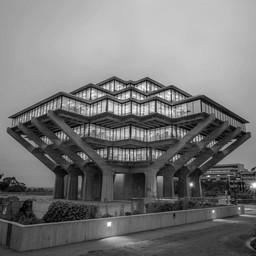
\includegraphics[scale=0.75]{true_ucsd}
        \caption{Test Image $1$ ($256\times 256$ pixels)}
        \label{fig:true}
    \end{subfigure}
    \hfill
    \begin{subfigure}[b]{0.495\textwidth}
        \centering
        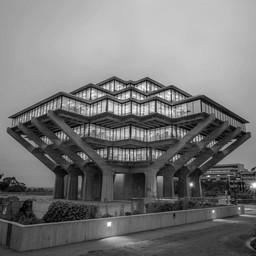
\includegraphics[scale=0.75]{recon_ucsd}
        \caption{Reconstructed Image (Rel. error $4.288\times 10^{-16}$)}
        \label{fig:recon}
    \end{subfigure}
    \vspace{0.05in} \\
    \begin{subfigure}[b]{0.495\textwidth}
        \centering
        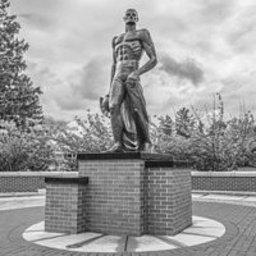
\includegraphics[scale=0.75]{true}
        \caption{Test Image $2$ ($256\times 256$ pixels)}
        \label{fig:true_msu}
    \end{subfigure}
    \hfill
    \begin{subfigure}[b]{0.495\textwidth}
        \centering
        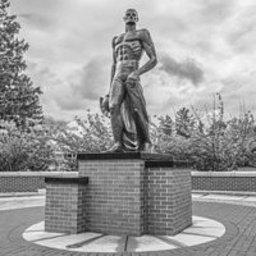
\includegraphics[scale=0.75]{recon}
        \caption{Reconstructed Image (Rel. error $2.857\times 10^{-16}$)}
        \label{fig:recon_msu}
    \end{subfigure}
    \vspace{0.05in}
    \caption{Two Dimensional Image Reconstruction from Phaseless Local Measurements.}
    \label{fig:2d-recon}
\end{figure}
%


We next plot the execution time (in seconds, averaged over $50$ trials) required to implement
Algorithm~\ref{Alg1} for different values of $d$ in Fig. \ref{fig:etime}. In each case, $\delta$ was
chosen to be $\lceil \log_2(d) \rceil$, with the same choice of measurement vectors as for the
reconstruction in Fig.  \ref{fig:recon}. The plot confirms that the proposed method is extremely
efficient; indeed, the plot reveals an FFT-time empirical computational complexity of $\mathcal
O(d^2 \log_2(d^2))$.

Finally, Fig. \ref{fig:noise} illustrates the robustness of the proposed method to measurement
errors (an analysis of noise robustness is omitted from the paper and should follow from an appropriate generalization of the techniques used for the analysis of BlockPR\cite{iwen2016phase} in the one-dimensional case). The figure plots the reconstruction error (averaged over $50$ trials) in reconstructing a
$64\times 64$ random matrix with i.i.d zero-mean complex Gaussian entries from phaseless
measurements (with $\delta=6$, and with the same measurement construction as with Fig.
\ref{fig:recon}). An additive noise model with i.i.d. zero-mean Gaussian noise was used to corrupt
the measurements. The added noise as well as reconstruction error are reported in decibels, with
%
\[  \text{SNR (dB)} = 10 \log_{10}\left( \frac{\Vert \y \Vert_2^2}{D\sigma^2}\right), \qquad 
    \text{Error (dB)} = 10 \log_{10} \left( \frac{\min_\theta\Vert \mathbbm 
                e^{\mathbbm i \theta}X-Q\Vert^2_F}{\Vert Q\Vert^2_F}\right). \]
%
%For added robustness, an improved eigenvector-based magnitude estimation method detailed in 
%\cite[Section 6.1]{iwen2016phase} was utilized in place of Step 4 of Algorithm~\ref{Alg1}. 
%We observe that the proposed algorithm demonstrates robustness across a wide variety of SNRs. Moreover, 
%the test signals are reconstructed to (almost) the level of added noise. 
We observe that the proposed algorithm (indicated by the dashed line) demonstrates robustness 
across a wide variety of SNRs. Additionally, the results from utilizing an improved
(eigenvector-based) magnitude estimation method (detailed in \cite[Section 6.1]{iwen2016phase}) 
in place of Step 4 of Algorithm~\ref{Alg1} is plotted using the solid line. In both cases, we
observe that the test signals are reconstructed to (almost) the level of added noise. 
%
\begin{figure}[hbtp]
    \centering
    \begin{subfigure}[b]{0.495\textwidth}
        \centering
        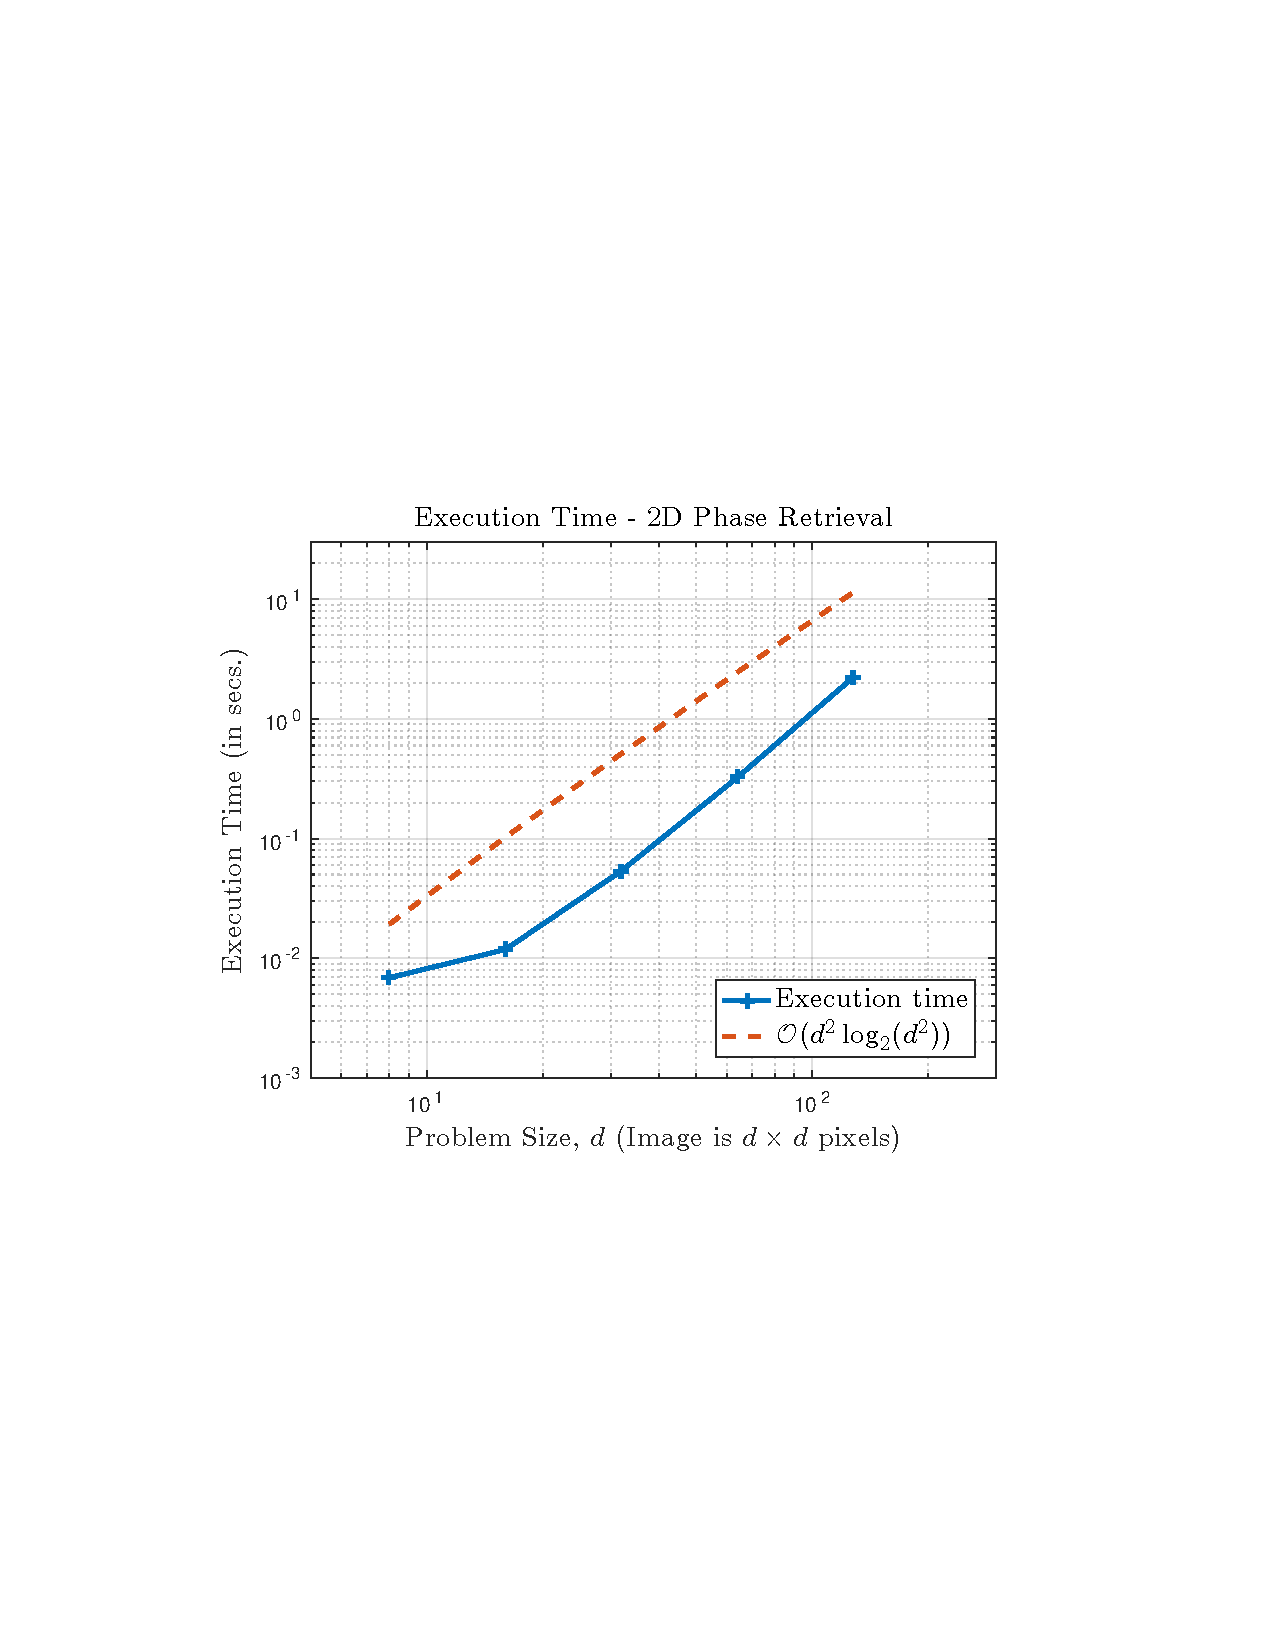
\includegraphics[clip=true, trim = 1.10in 3.25in 0.75in 3.25in,
scale=0.55]{etime}
        \caption{Execution Time vs Problem Size}
        \label{fig:etime}
    \end{subfigure}
    \hfill
    \begin{subfigure}[b]{0.495\textwidth}
        \centering
        %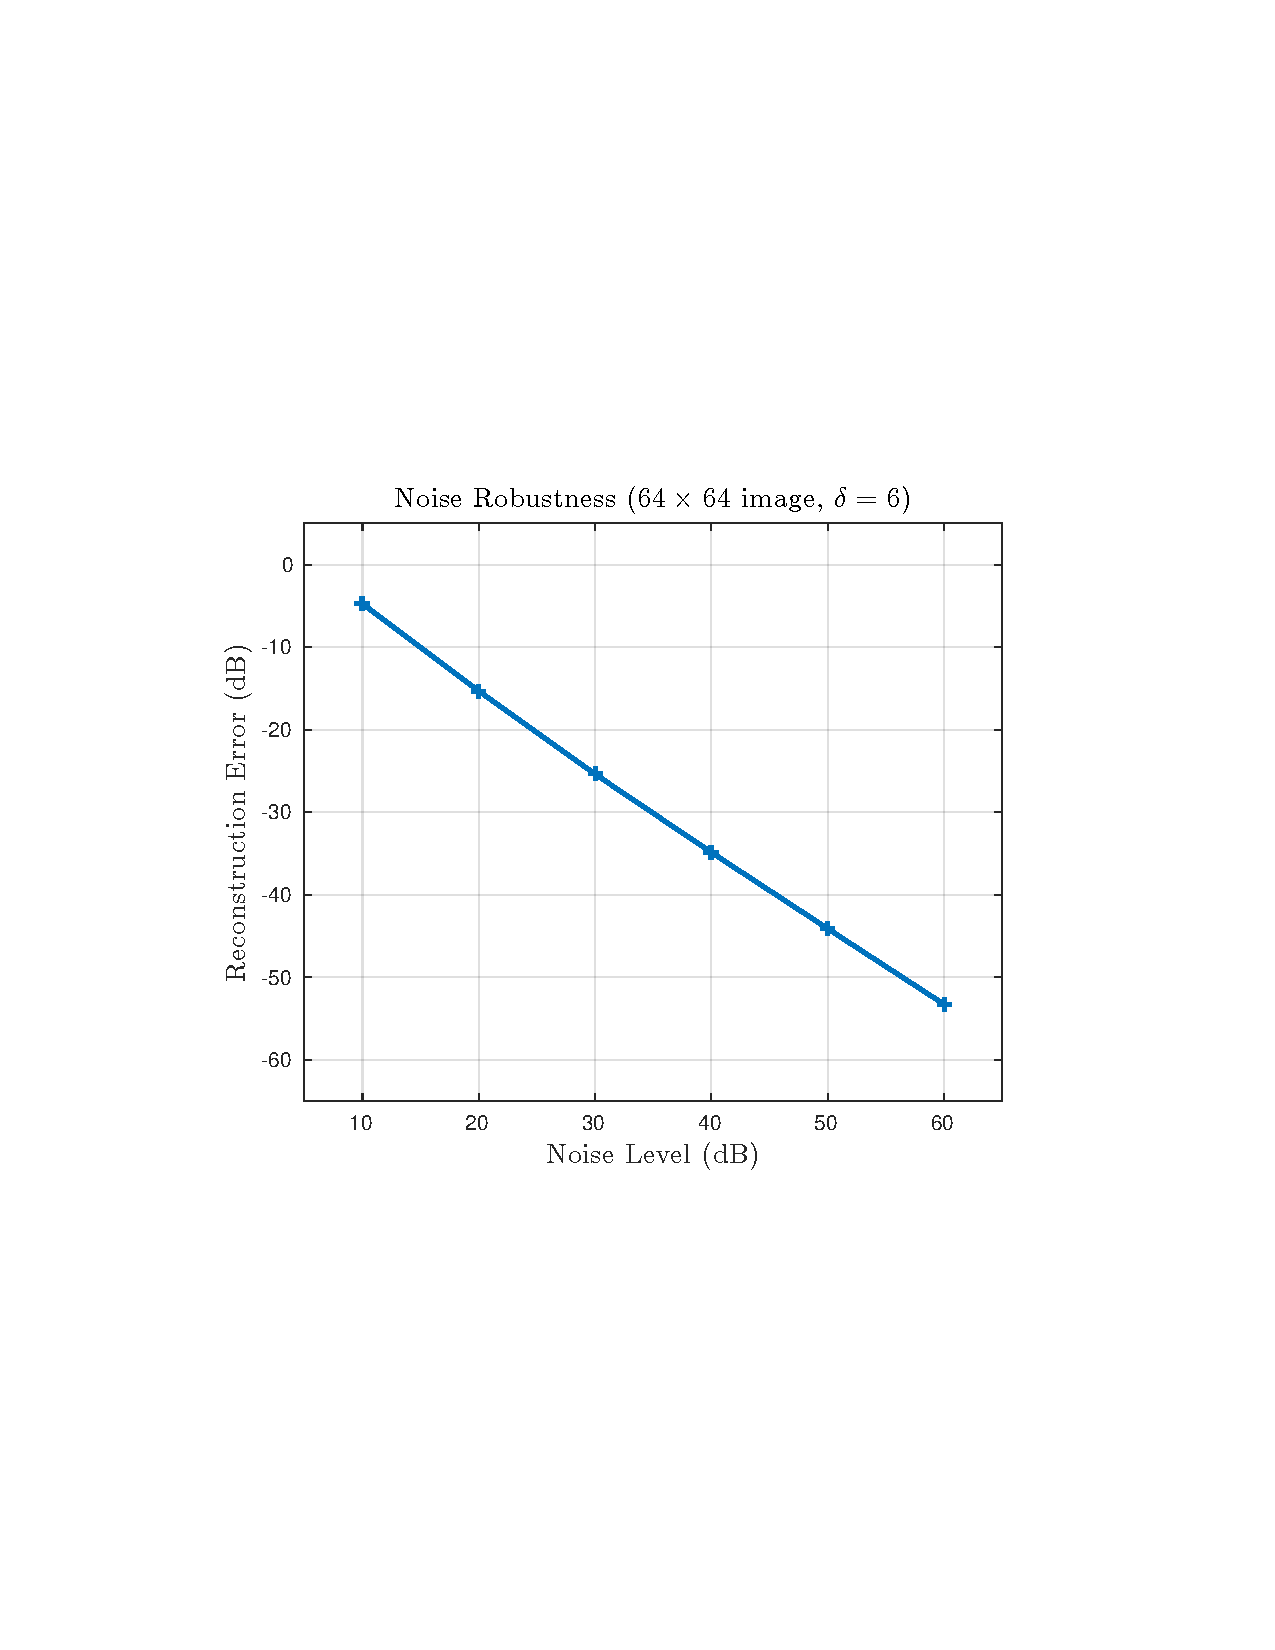
\includegraphics[clip=true, trim = 1.10in 3.15in 0.75in 3in,scale=0.55]{noise}
        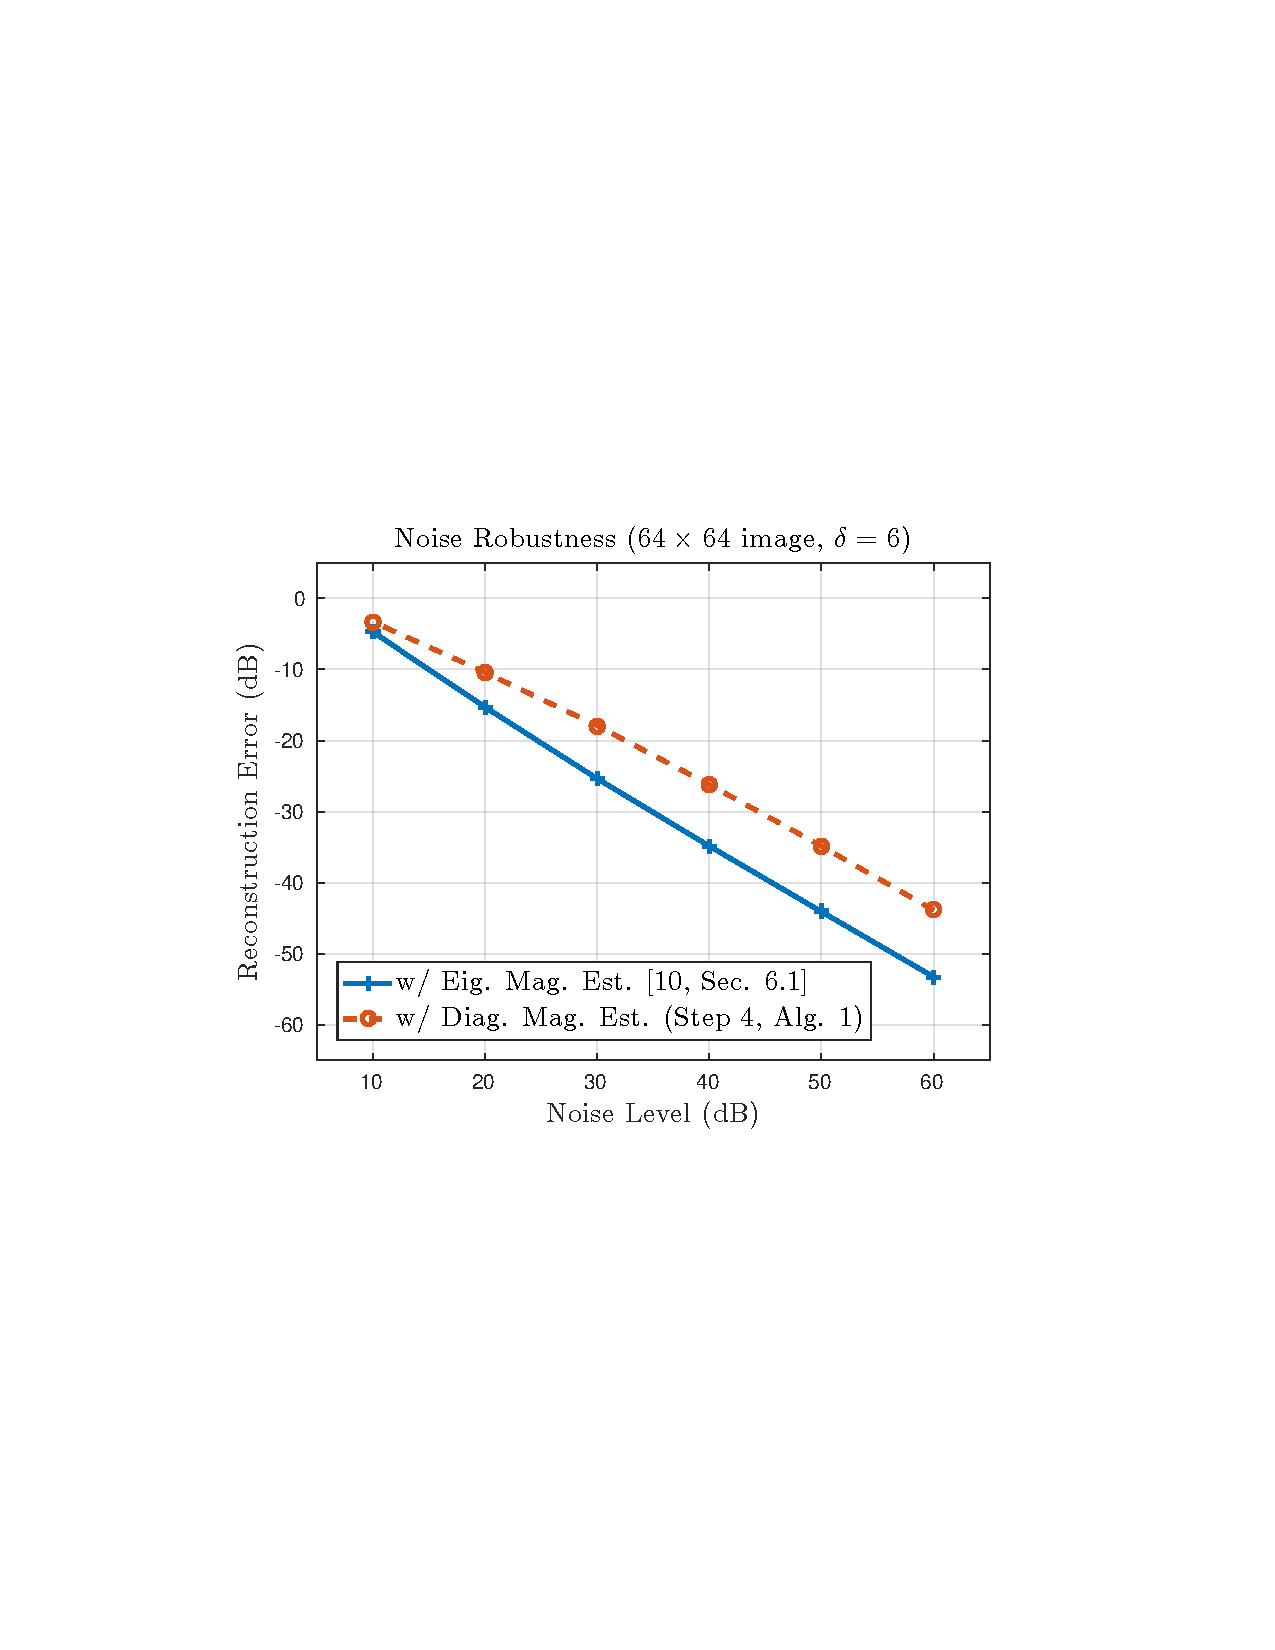
\includegraphics[clip=true, trim = 1.10in 3.25in 0.75in 3in,scale=0.575]{noise_alt}
        \caption{Noise Robustness of the Proposed Method}
        \label{fig:noise}
    \end{subfigure} 
    \vspace{0.05in}
    \caption{Evaluating the Efficiency and Robustness of the Proposed Two Dimensional Phase
    Retrieval Algorithm.}
    \label{fig:perf}
\end{figure}
%



\acknowledgments % equivalent to \section*{ACKNOWLEDGMENTS}       
 
This work was supported in part by NSF DMS-1416752 and NSF DMS-1517204, as well as a UCSD  Academic Senate Research Grant. % References
Parts of the numerical simulations were performed while the first and last authors were visiting the 
Institute for Computational and Experimental Research in Mathematics (ICERM), Brown University,
Providence, RI.

\bibliography{refs} % bibliography data in report.bib
\bibliographystyle{spiebib} % makes bibtex use spiebib.bst


\end{document}
